\documentclass[10pt,a4paper]{article}

\newcommand{\COLORSDIR}{/Users/hoolywear/Desktop/UNIMORE/II ANNO/II SEMESTRE/colors}

\usepackage[italian]{babel}
\usepackage[usenames,dvipsnames,table]{xcolor}
\usepackage[utf8]{inputenc}
\usepackage[T1]{fontenc}
\usepackage{soul}
\usepackage[a4paper, portrait, margin=2.5cm]{geometry}
\usepackage{array}
\usepackage{tabularx}
\usepackage{multicol}
\usepackage{amsmath}
\usepackage{amsfonts}
\usepackage{amssymb}
\usepackage{algorithmicx}
\usepackage[noend]{algpseudocode}
\usepackage{wrapfig}
\usepackage{graphicx}
\usepackage{hyperref}
\hypersetup{
    colorlinks=true,
    linkcolor=black,
    filecolor=magenta,      
    urlcolor=cyan,
    pdftitle={Overleaf Example},
    pdfpagemode=FullScreen,
    }
\urlstyle{same}
\usepackage{caption}
\usepackage{capt-of}
\captionsetup[figure]{name=Fig.}
\renewcommand{\thefigure}{\arabic{section}.\arabic{figure}}
\graphicspath{ {./images/} }

\input{\COLORSDIR/colors_4}

\usepackage{listings}

\definecolor{codeblue}{HTML}{1e66f5}
\definecolor{codepurple}{HTML}{8839ef}
\definecolor{codered}{HTML}{d20f39}
\definecolor{darkbluenord}{HTML}{232731}
\definecolor{lightbluenord}{HTML}{b1bfe3}

\lstdefinestyle{code}{
    backgroundcolor=\color{gray!10},   
    basicstyle=\ttfamily,
    commentstyle=\color{codeblue},
    keywordstyle=\color{codered},
    breakatwhitespace=false,         
    breaklines=true,                 
    captionpos=b,                    
    keepspaces=true,                 
    showspaces=false,                
    showstringspaces=false,
    showtabs=false,                  
    tabsize=2,
    mathescape=true %dollar signs act as inline math delimiters
}

\lstdefinestyle{python}{
    style=code,
    language=python,
    commentstyle=\color{codeblue},
    keywordstyle=\color{codepurple},
    stringstyle=\color{codered}
}

\lstset{style=code,language=C++}

\usepackage[framemethod=TikZ]{mdframed}

\mdfsetup{%
  roundcorner=8pt}

% styles
\def\Clinewidth{.8pt}
\mdfdefinestyle{titlerule}{%
  frametitlerule=true,%
  frametitlerulewidth=\Clinewidth,%
  subtitleaboveline=true,subtitlebelowline=true,%
  subtitleabovelinewidth=\Clinewidth,subtitlebelowlinewidth=\Clinewidth,%
linewidth=1pt}

\mdfdefinestyle{emphasize}{%
  style=titlerule,%
  frametitle=,%
  linecolor=gray!50,linewidth=1pt,backgroundcolor=gray!10}

% algorithmic environment
\surroundwithmdframed[backgroundcolor=gray!10,hidealllines=true,%
frametitle={}]{algorithmic}

% quote environment
\surroundwithmdframed[style=emphasize]{quote}

% example environment
\newmdenv[frametitle=Esempio,style=titlerule]{example}

% emphasize environment
\newmdenv[style=emphasize,%
          linecolor=emp!70!red,backgroundcolor=emp]{emphasize}

% blue emphasize environment
\newmdenv[style=emphasize,%
          linecolor=obs!70,backgroundcolor=obs!20]{emphasize-blue}

%% NOT USED IN III ANNO
%% % definition environment
%% \newmdenv[frametitle=Definizione,style=titlerule,%
%%           linecolor=def]{definition}
%% 
%% % theorem environment
%% \newmdenv[frametitle=Teorema,style=titlerule,%
%%           linecolor=the]{theorem}
%% % observation environment
%% \newmdenv[frametitle=Osservazione,%
%%           backgroundcolor=white,linecolor=obs,%
%%           frametitlebackgroundcolor=obs]{observation}
%% 
%% % warning environment
%% \newmdenv[style=emphasize,%
%%           backgroundcolor=war!10,linecolor=war]{warning}

\author{Iacopo Ruzzier}
\date{Ultimo aggiornamento: \today}


\title{%
Compilatori\\
\large Parte Due}

\begin{document}
\maketitle
\tableofcontents
\newpage
\section{Introduzione (25 feb)}

\subsection{Motivazione}

Ricordiamo il ruolo del compilatore tra le tecnologie informatiche, quello dell'ISA e del linguaggio assembly, i passaggi gestiti dal compilatore, dall'assembler, eccetera
\begin{itemize}
  \item Il compilatore \textbf{traduce un programma sorgente in linguaggio macchina}
  \item L'ISA agisce da "interfaccia" tra HW e SW (fornisce a SW il set di istruzioni, e specifica a HW che cosa fanno)
\end{itemize}

\subsubsection{La funzione dei compilatori}

\begin{itemize}
  \item Funzione principale e pi\`u nota: trasformare il codice \textbf{da un linguaggio ad un altro} (es. C $\rightarrow$ Assembly RISC-V) (ricordiamo che \`e solo il primo passo di un'intera toolchain di programmi per creare eseguibili)

\item Gestendo la traduzione a linguaggio macchina al posto dei programmatori, l'altra funzione importante \`e l'\textbf{ottimizzazione} del codice, che permette la \textbf{produzione di eseguibili di stesse funzionalit\`a}, ma diversi a livello di \textbf{dimensioni} (es. per sistemi embedded e high-performance), \textbf{consumo energetico}, \textbf{velocit\`a di esecuzione}, ma anche in termini di determinate \textbf{caratteristiche architetturali} utilizzate (es. proc.~multicore)
\end{itemize}

\subsubsection{L'evoluzione dei compilatori}

Le rivoluzioni in termini di "classe" di dispositivi e di dimensioni dei transistor sono molto frequenti (Bell, Moore), e nei primi 2000 si arriva ai \textbf{limiti fisici della miniaturizzazione e della frequenza} operativa dei processori (e conseguenti problemi di dissipazione del calore prodotto) $\rightarrow$ nasce l'idea di cambiare completamente il paradigma di sviluppo di un processore: dal singolo core sempre pi\`u potente passo a \textbf{pi\`u core "isopotenti"} sullo stesso chip

\noindent\begin{minipage}[c]{.3\textwidth}
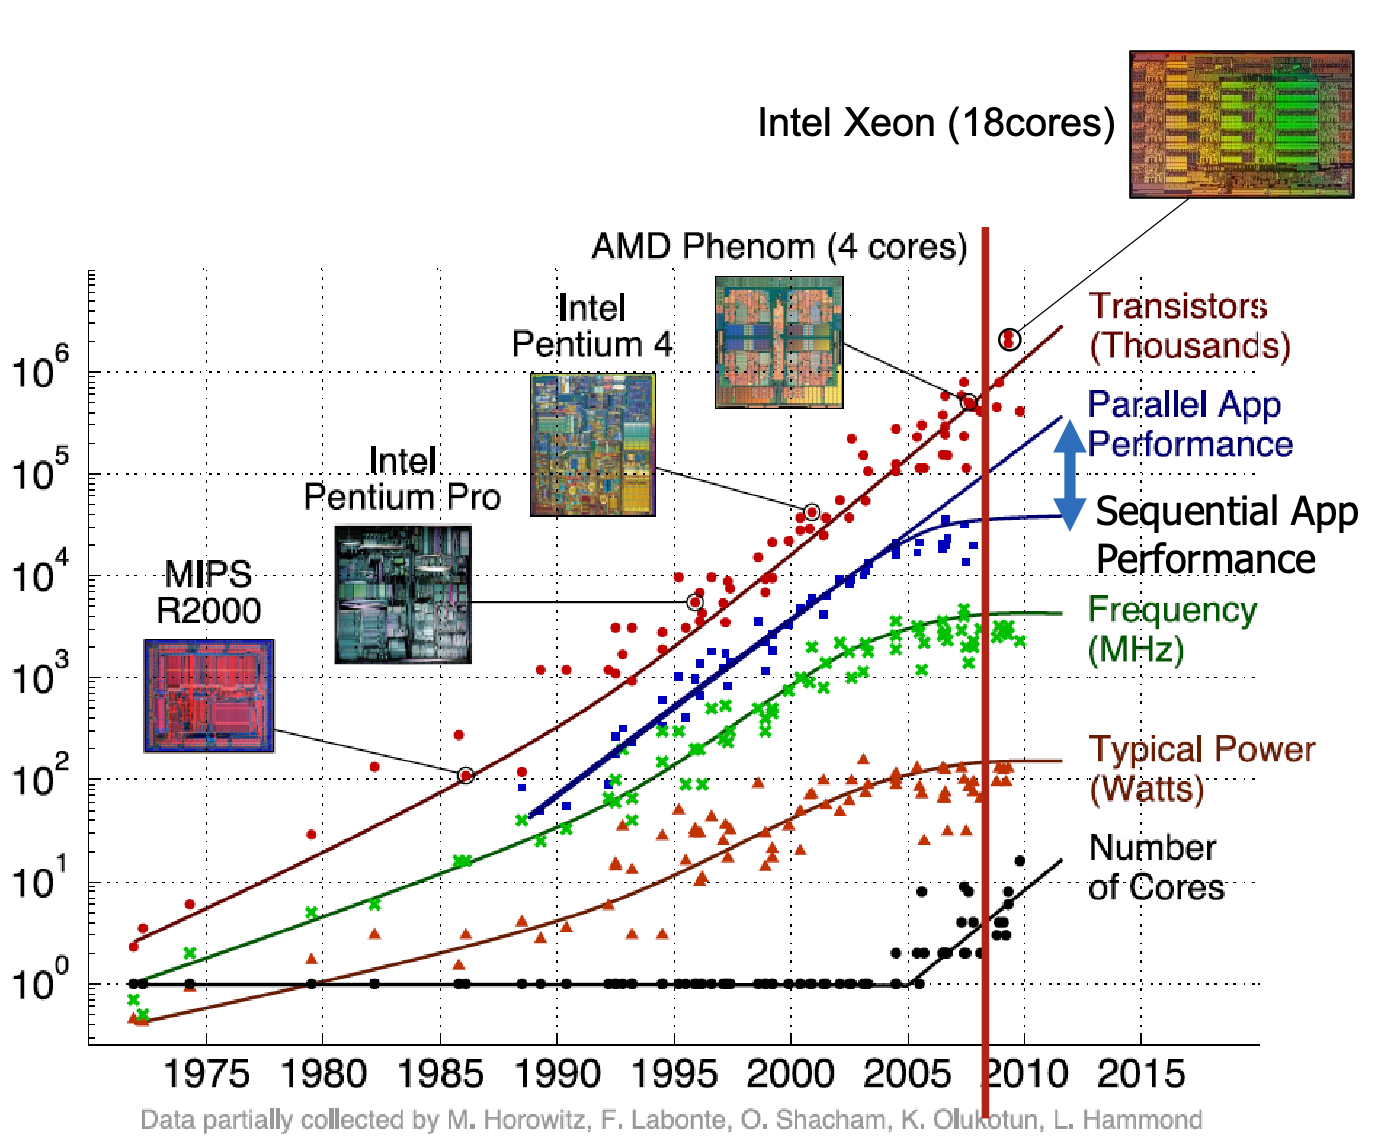
\includegraphics[width=\textwidth]{intro_1.png}
\end{minipage}
\begin{minipage}[c]{.7\textwidth}
  Notiamo come dal 2005 circa si raggiunge un plateau in termini di consumo, di frequenza e di performance di programmi \textit{sequenziali}, e aumenta la performance di programmi che \textbf{sfruttano la parallelizzazione} $\rightarrow$ i programmi devono essere "consapevoli" che il processore \`e multicore! Qui capiamo l'impatto dello sviluppo tecnologico sull'evoluzione dei compilatori
\end{minipage}

\begin{emphasize}
  Per evitare un cambio nella formazione dei programmatori, le aziende sperano nei compilatori autoparallelizzanti - non sar\`a mai possibile e nel mentre sono stati introdotti molti paradigmi di pr.~parallela
\end{emphasize}

Il compilatore mantiene un ruolo fondamentale: oltre a rendere meno "traumatico" il passaggio alla programmazione parallela, si interfaccia con i nuovi paradigmi di programmazione parallela offerti ai programmatori: il programmatore sfrutta interfacce semplici e astratte, mentre il compilatore traduce i costrutti in codice parallelo eseguibile (es. OpenMP)

\subsubsection{Eterogeneit\`a architetturale}

La programmazione parallela e il parallelismo architetturale sono oggi paradigmi consolidati, e i processori general purpose (seppur multicore e ottimizzati) non sono sufficienti per alcune attivit\`a specializzate come la grafica $\rightarrow$ nascono componenti \textbf{acceleratori} di vario tipo: GPU, GPGPU, FPGA, TPU, NPU...
Questo complica ulteriormente la scrittura del software, e dunque impone altre evoluzioni nei compilatori e nelle ottimizzazioni.

\subsection{Ottimizzazione}

Ricordiamo le metriche usate:

\noindent\begin{minipage}[c]{.5\textwidth}
\begin{equation*}
  \text{Performance} = {{1}\over\text{Execution Time}}
\end{equation*}
\end{minipage}
\begin{minipage}[c]{.5\textwidth}
\begin{equation*}
  \text{Execution Time} = {\textcolor{blue}{\text{Instruction Count}} \times \textcolor{red}{\text{CPI}} \over \textcolor{red}{\text{Frequency}}}
\end{equation*}
\end{minipage}\\

Le ottimizzazioni possono avvenire dal punto di vista \textcolor{red}{HW (parametri architetturali)} e da quello \textcolor{blue}{SW (p.~di programma)}. Il compilatore pu\`o agire anche ad es. a livello di cache, aiutando a ridurre i miss e dunque i CPI delle istruzioni \lstinline|load| e \lstinline|store|

\subsubsection{Esempi di ottimizzazione}

\begin{emphasize}
  Distinguiamo le ottimizzazioni che avvengono a compile time o a runtime (statiche o dinamiche)
\end{emphasize}

\begin{itemize}
  \item AS (Algebraic Semplification): ottimizzazione a runtime
  \begin{lstlisting}
-(-i) $\rightarrow$ i
b or true $\rightarrow$ true //cortocircuito logico\end{lstlisting}
  \item CF (Constant Folding):  valutare ed espandere espressioni costanti a compile time
  \begin{lstlisting}
c = 1+3 $\rightarrow$ c = 4
(100<0) $\rightarrow$ false\end{lstlisting}
  
  \item SR (Strength Reduction): sostituisco op. costose con altre pi\`u semplici: classico es. MUL rimpiazzate da ADD/SHIFT (dobbiamo ovviamente tenere conto delle implementazioni hw delle operazioni): esempi a slide 30\\
  esempio sofisticato: for con operazioni su array, sostituito da operazioni su puntatori (aritmetica dei pt.) $\rightarrow$ il risultato si vede nel codice assembly (riporta listings)
\item CSE (Common Subexpression Elimination): elimino i calcoli ridondanti di una stessa espressione riutilizzata in pi\`u istruzioni (statement)
\item DCE (Dead Code Elimination): elimino tutte le istruzioni che producono codice mai letto (e dunque utilizzato), es. variabili assegnate e mai lette, codice irraggiungibile $\rightarrow$ uno dei passi eseguiti pi\`u di frequente durante l'ottimizzazione del codice da parte del compilatore, per rimuovere anche tutto il dead code generato dagli altri passi di ottimizzazione
\item Copy Propagation: per uno statement \lstinline|x = y|, sostituisco gli usi futuri di \lstinline|x| con \lstinline|y| se non sono cambiati nel frattempo (propedeutico alla DCE)
\item CP (Constant Propagation): sostituisco usi futuri di una variabile con assegnato valore costante con la costante stessa (se la variabile non cambia) (slide 38 esempio di sequenza di ottimizzazioni applicate in sequenza) (stiamo sempre ipotizzando che i valori a fine esempi siano poi \textbf{utilizzati}, e non dead code)
\item LICM (Loop Invariant Code Motion): si occupa di muovere fuori dai loop tutto il codice \textbf{loop invariant}; evita i calcoli ridondanti\\
\begin{lstlisting}
while (i<100) {
  *p = x/y + i;
  i = i + 1;
}
\end{lstlisting}
diventa
\begin{lstlisting}
t = x + y;
while (i < 100) {
  *p = t + i;
  i = i + 1;
}
\end{lstlisting}
recupera questione su load e store, questione su CPI medio per una load e quando si riduce/ arriva a 1 (quando si trova in cache, di solito ordine delle decine)\\
chiedi a dani

\end{itemize}

\subsubsection{Ottimizzazioni sui loop}

\begin{itemize}
  \item grande impatto sulla performance dell'intero programma (per ovvie ragioni)
  \item spesso sono ottimizzazioni propedeutiche a quelle machine-specific (effettuate nel backend): register allocation, instruction level parallelism, data parallelism, data-cache locality
  \item sono in generale target delle ottimizzazioni, essendo centrali per il parallelismo
\end{itemize}

\subsection{Anatomia di un compilatore}

Un compilatore svolge almeno due compiti: analisi del sorgente e sintesi di un programma in linguaggio macchina; lo fa operando su una rappresentazione intermedia (IR) che si interpone tra frontend e backend, e tra source code e target code

il blocco di middle-end agisce sul codice intermedio, e in vari passaggi lo trasforma  e lo ottimizza (diverso a seconda del compilatore)

caso llvm: clang (frontend) $\rightarrow$ opt (middleend) $\rightarrow$ llc (backend)

l'ottimizzatore opt si basa su una serie di \textbf{passi di ottimizzazione (o di analisi)}: un passo di analisi scorre l'IR e lo analizza (non lo trasforma, ma produce informazioni utili); un passo di ottimizzazione sfrutta informazioni conosciute per trasformare l'IR (applica le ottimizzazione)


alcune ottimizzazioni non possono essere effettuate o finalizzate senza conoscere l'architettura target (es. sulle cache), e dunque vengono eseguite dal backend

\subsubsection{Flag di ottimizzazione}

sono flag che passo al compilatore (al pass manager) per influenzare \textbf{ordine e numero dei passi di ottimizzazione}
\begin{itemize}
  \item \lstinline|-g|: solo debugging, nessuna ottimizzazione
  \item \lstinline|-O0|: nessuna ottimizzazione
  \item \lstinline|-O1|: solo ott. semplici
  \item \lstinline|-O2|: ott. pi\`u aggressive
  \item \lstinline|-O3|: esecuzione dei passi in un ordine che sfrutta compromessi tra velocit\`a e spazio occupato
  \item \lstinline|-OS|: ottimizza per dimensione del compilato
\end{itemize}

\subsubsection{Uso di IR}

un backend che fa uso di IR permette di disaccoppiare con facilit\`a frontend e backend, lavorare su ottimizzazioni machine-independent, semplificare il supporto per molti linguaggi, eccetera

\begin{emphasize}
  Per supportare un nuovo linguaggio o una nuova architettura, basta scrivere un nuovo front/backend - il middle-end pu\`o rimanere lo stesso!
\end{emphasize}

\subsubsection{Ingredienti dell'ottimizzazione}

slide 49-51

\section{Rappresentazione intermedia (4 mar)}

ricordiamo: middle end come sequenza di passi, di analisi o di trasformazione $\rightarrow$ per analizzare e trasformare il codice occorre una rappr.~intermedia (IR) \textbf{espressiva} che \textbf{mantenga le informazioni importanti da un passo all'altro}

\subsection{propriet\`a di una IR}

scegliamo IR diverse a seconda del loro uso, in generale alcune caratteristiche sono sempre richieste:
\begin{itemize}
  \item facilita di generazione (effetti sul frontend)
  \item facilita e costo di manipolazione
  \item livello di astrazione e di dettaglio esposto: effetti sul frontend e sul backend (diverse IR da un lato e dall'altro, a seconda del livello di astraz.~e di dettaglio necessari)
\end{itemize}

\subsection{Tipi di IR}

\begin{itemize}
  \item AST (abstract syntax tree)
  \item DAG (grafi diretti aciclici)
  \item 3-address code (3AC): assomiglia molto all'assembly (3 indirizzi in quanto registro destinazione e max2 operandi)
  \item SSA (Static Single Assignment): evoluzione di 3ac con ulteriori propriet\`a di control flow (?)
  \item CFG (control flow graphs)
  \item CG (call graph)
  \item PDG (program dependence graphs)
\end{itemize}

call graph: rappresenta "come" vengono chiamate le funzioni (a partire dal main)

ottimizzazioni inter-procedurali: devono per forza basarsi su IR di tipo cg (es. per decidere quando fare INLINING - espandere il codice della funzione invece di chiamarla - evidente tradeoff tra dimensione del codice e overhead dovuto alla chiamata di funzione)

pdg: rappresentazione fondamentale per lavorare sul parallelismo, multithreading eccetera

\subsection{categorie di IR}

\begin{itemize}
  \item grafiche (o strutturali)
    \begin{itemize}
      \item orientate ai grafi
      \item molto usate nella source-to-source translation: uso tipico - ottimizzazioni che non hanno bisogno della struttura sofisticata di un middle-end (es. openMP: sono di fatto delle annotazioni sul codice, dunque lo scopo principale di questo programming model \`e fornire uno strumento semplice al programmatore (es. outlining: prendo es un loop e lo impacchetto in una funzione che poi dovra essere eseguita dai thread per la parallelizzazione) - dunque in questo caso non sto ottimizzando nel senso proprio del termine, ma sto trasformando il codice e lo sto rendendo eseguibile in maniera parallela - mi bastsa un IR di questa categoria)
      \item solitamente voluminose (basate su grafi) - tradeoff con il fatto che sono usate prima del middle-end (senza doverlo coinvolgere)
      \item es. ast, dag
    \end{itemize}
  \item lineari
    \begin{itemize}
      \item pseudocodice per macchine astratte
      \item livello di astrazione vario
      \item strutture dati semplici e compatte
      \item facile da riarrangiare (evidentemente il piu comodo per eseguire le ottimizzazioni)
      \item es. 3ac
    \end{itemize}
  \item ibride (sfruttano combinazioni delle prime due) (es cfg)
\end{itemize}
\subsection{esempi di rappresentazione}


\subsubsection{sintassi concreta (testo)}

maniera piu semplice in quanto piu vicina al livello di astrazione "umano" di ragionamento sul programma, ma non il livello corretto per ottimizzare ne comprendere correttamente la semantica del programma

\begin{lstlisting}[language=java]
let value = 8;
let result = 1;
for (let i = value; i>0; i = i - 1) {
  result = result * i;
}
console.log(result);\end{lstlisting}

\subsubsection{ast}

albero i cui nodi rappresentano diverse parti del programma, con il nodo radice che rappresenta il \textbf{programma}, il quale a sua volta contiene un blocco di istruzioni dal quale discendono tanti figli quante le sue istruzioni

esempi immagini

pro: molto comodo per interpreti (basta usare fz ricorsiva per processare l'albero)

contro: un nodo \`e un oggetto troppo generico $\rightarrow$ analizzare un ast per l'ottimizzazione impone ogni volta di ragionare sulla differenza semantica tra i nodi (complica molto)

\subsubsection{dag (digressione)}

contrazione di ast che evita la duplicazione di espressioni $\rightarrow$ rappresentazione piu compatta

limite: il riuso e possibile solamente dimostrando che il suo valore non cambia nel programma $\rightarrow$ essendo assegnamenti e chiamate frequentissimi, evidentemente il fatto che il dag non abbia nozione di come le espr cambino valore nel tempo non lo rende un buon candidato per le ottimizzazioni

\begin{example}
   codice generato da questo dag corretto?
%   \begin{lstlisting}
%x = a + a * (b – c)
%y = (b – c ) * d
%z = x + y
%# espressioni trovate
%t1 = b – c
%t2 = a * t1
%x = a + t2
%y = t1 * d
%z = x + y
%   \end{lstlisting}
corretta, mentre per altro esempio no   
\end{example}



\subsubsection{3ac}

evidentemente adatto alle ottimizzazioni: tutte le istruzioni del programma vengono spezzettate in istruzioni di forma semplice simile all'assembly

in questo caso istr di tipo \lstinline|x = y op z| (1 operatore, massimo 3 operandi)

esempio:

\lstinline|x - 2 * y| $\rightarrow$ \lstinline|t1 = |

pro: espressioni complesse spezzettate, forma compatta e simile a assembly
introdotti registri temporanei intermedi, virtuali e illimitati (non mi preoccupo dei problemi architetturali di quanti registri fisici ho a disposizione, sono a livello decisamente piu alto - le eventuali op. di spill (aggiungere load o store in mncanza di registri fisici) non le gestisco qui)

rec

\paragraph{varianti di 3ac}~\\

varianti a seconda dei vincoli che ho per l'implementazione pratica

quadruple: id istruzione, opcode, i 3 registri (semplice struttura record, facile da analizzare e riordinare ma i nomi espliciti prendono pi\`u spazio)
triple: id istruzione, opcode, 2 operandi $\rightarrow$ uso l'indice dell'espressione nell'array come "nome" del registro destinazione $\rightarrow$ risparmio spazio, ma diventa piu complesso da analizzare (nomi impliciti) e soprattutto da riordinare


ricordiamo la constant propagation: sostituisco usi futuri di una variabile con valore costante con la costante stessa \textbf{se non cambia nel frattempo}

$\rightarrow$ ottimizzazione che una IR di tipo 3ac non puo applicare immediatamente (devo prima analizzare il resto del codice) $\rightarrow$ SSA come evoluzione della 3ac, in quanto impone che la \textbf{definizione (assegnamento)} delle variabili avvenga \textbf{solo una volta} (definizioni multiple sono tradotte in multiple versioni della var)

pro: ogni definizione ha associata direttamente una lista di tutti i suoi usi - semplifica enormemente le ottimizzazioni di tipo CP e non solo

quasi sempre uno dei passi di ottimizzazione prevede il passaggio a forma SSA

\subsection{scelta della IR}

dipende ovviamente dal livello di dettaglio necessario per ogni specifico compito - in un compilatore coesistono piu IR

anche per questo ci sono le forme ibride - es. cfg con 3ac

\subsubsection{cfg}

vediamo un esempio con costrutti condizionali (non solo sequenze lineari)

immagine slide 2-28

un cfg permette di aggiungere informazioni sui \textbf{salti} al di sopra di una IR lineare $\rightarrow$ modello il flusso di controllo del programma come grafo composto da blocchi (BB)

ogni bb contiene sequenze lineari di istruzioni

gli archi rappresentano il flusso di controllo del programma


formalmente: un BB \`e una seq.~di istruzioni in forma 3AC
\begin{itemize}
  \item solo la prima istruzione puo essere raggiunta dall'esterno (garantito un singolo entry point)
  \item singolo exit point: se eseguo la prima istr.~\textbf{devo eseguire tutte le altre} - garantisco che venga eseguito interamente
\end{itemize}

le chiamiamo sezioni single-entry, single-exit (possono essere sezioni anche piu grandi, ma le piu piccole di questo tipo sono i BB)

un arco connette due nodi s.s.se il secondo puo eseguire dopo il primo in qualche percorso del ctrl flow del programma (prima istr del secondo \`e target dell'istr di salto al termine del primo, oppure il secondo \`e l'unico successore del primo che non ha un istr di salto come ultima istr - il secondo lo chiamo nodo falltrough)

un cfg \textbf{normalizzato} ha i bb \textbf{massimali} (non possono essere resi piu grandi senza violare condizioni) (unisco i bb fallthrough che non hanno label all'inizio, evidentemente) (situazioni di cfg non normalizzato possono avvenire dopo qualche generico passo di ottimizzazione, evidentemente non le facciamo accadere noi "spontaneamente")

\paragraph{algoritmo per la costruzione del cfg}~\\

\begin{enumerate}
  \item identificare il \textbf{leader} di ogni bb:
    \begin{itemize}
      \item la prima istruzione
      \item il target di un salto
      \item ogni istruzione dopo un salto
    \end{itemize}
  \item il bb comincia con il leader e termina con l'istruzione immediatamente precedente un nuovo leader (o l'ultima istruzione)
  \item connettere i bb tramite archi di 3 tipi:
    \begin{itemize}
      \item fallthrough (o fallthru): esiste solo un percorso che collega i due blocchi
      \item true: il secondo blocco \`e raggiungibile dal primo se un condizionale \`e true
      \item false: il secondo blocco \`e raggiungibile dal primo se un condizionale \`e false
    \end{itemize}
    
\end{enumerate}

esempi ed esercizi fino slide 52

\subsubsection{dependency graph}

soprattutto nell'erad ei nulticore questa rappr assume sempre piu importanza

almeno due tipi: (recupera questa cosa)

ricordiamo pipeline riscv e data hazard: il fatto che un registro voglia leggere da un registro usato in un'op precedente (e non ancora salvato? recupera)

if id exe mem wb le fasi di pipelining

esempio con una mul: ricordiamo che se la mul successiva prova a usare il registro usato nell'istr prima (dipendenza), il risultato ancora non e stato scritto - nella fase di decode identifico i registri usati nell'operazione, e appunto rw ancora non contiene il risultato aggiornato, che sara pronto appena tra 2 cicli

questo e un data hazard, nel caso comune si gestisce con una \textbf{forwarding unit} che bypassa le fasi successive e inoltra direttamente il risultato appena ottenuto

per quanto la fw unit sia un pezzo di hw dedicato che fa questi controlli autonomamente, in generale l'unico modo per evitare questo tipo di hazard \`e distanziare abbastanza le istruzioni tra loro affinche il dato sia disponibile $\rightarrow$ sposto l'istruzione di mul inserendo nop (cicli di stallo) (evidentemente non buono - vado a "rompere" l'IPC paria a 1 della pipeline sempre piena, evidentemente diminuisce la performance)

soluzione migliore: scheduling del programma, ovvero sposto istruzioni che non hanno bisogno di quei registri per riempire quello spazio altrimenti occupato necessariamente da nop

questo \`e uno dei compiti principali di un backend - \textbf{in che ordine genero le istruzioni per massimizzare l'efficienza del programma}

come faccio a fare questa cosa? manualmente: vado a guardare le istruzioni e cerco a mano le dipendenze; il backend sfrutta la IR di tipo dg che fornisce esattamente le informazioni sulle dipendenze tra istruzioni

qui si capisce cosa si intende per instruction level parallelism: dunque, quando \`e possibile sfruttare tutte le parti di architettura per "parallelizzare il codice" anche in caso di single thread (ottimizzazione senza reale parallelismo)


\subsubsection{data dependency graph ddg}

specifico per multicore e parallelismo, usato per dare una rappresentazione tra le dipendenze dei \textbf{dati} - tipicamente i loop

per esempio, loop innestati lavorano tipicamente su str dati complesse e multidimensionali (matrici, immagini, eccetera)

esempio: for i = 0, i < n, i++
A[i]=init()

in questo caso \`e evidente come ogni iterazione resta indipendente dalle altre (uso il solo indice del loop)

sufficiente aggiungere qualcosa come A[i-1] = A[i] per generare dipendenze tra le iterazioni

di fatto mi sta dicendo che questo loop non \`e parallelizzabile in nessun modo, e deve per forza essere eseguito in sequenza

evidentemente le casistiche reali sono molto pi\`u complesse $\rightarrow$ esistono vari modi per rappresentare lo spazio delle iterazioni di un loop e le dipendenze che ne derivano

modello usato all'oggi: polyhedral model $\rightarrow$ rappresento lo spazio delle it.~come un poliedro (a seconda del numero di loop innestati), che permette di capire se esiste qualche permutazione dei loop (direzione di attraversamento dello spazio delle iterazioni; ovvero ad esempio scambiare l'ordine dei loop) non soggetta a dipendenze

\subsubsection{call graph}

rappresetnazione grafica a grafo usata per ragionare sulle relazione tra le funzioni della translation unit del file (insieme delle potenziali chiamate tra funzioni)

rappr.~gerarchica, utile soprattutto a livello di analisi \textbf{interprocedurale} (la maggior parte delle ottimizzazioni avvengono a livello intraprocedurale) (recupera questo concetto) (lavora sui file che abbiamo chiamato translation units, ovvero quelli da cui poi genero i file oggetto)

$\rightarrow$ evidente come il compilatore abbia visibilita solo fino a livello dei singoli moduli: posso estendere le ottimizzazioni al massimo fino ai legami tra funzioni dello stesso modulo - le ottimizzazioni piu ampie si spostano a framework di ottimizzazione che agiscono a livello di linker per esempio

\end{document}
